% Important: If latex complains about unicode characters,
% please use "\usepackage[utf8x]{inputenc}" in your preamble
% You can change the size of the picture by putting it into the construct:
% 1) \resizebox{10cm}{!}{"below picture"} to scale horizontally to 10 cm
% 2) \resizebox{!}{15cm}{"below picture"} to scale vertically to 15 cm
% 3) \resizebox{10cm}{15cm}{"below picture"} a combination of above two
% It is not recomended to use the scale option of the tikzpicture environment.
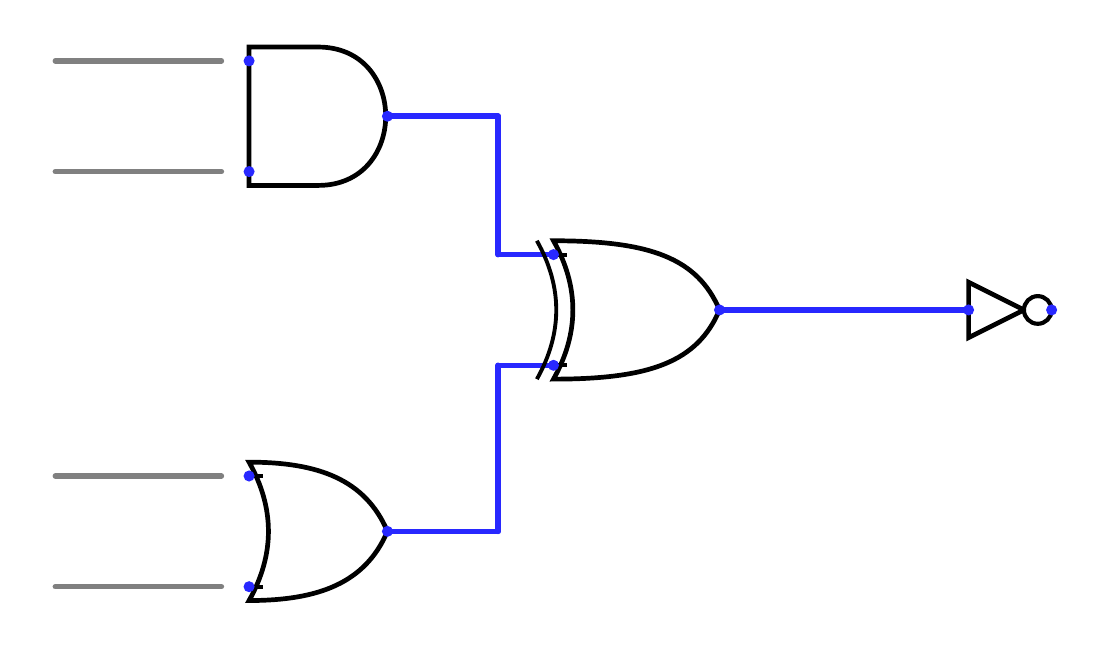
\begin{tikzpicture}[x=1pt,y=-1pt,line cap=rect]
\definecolor{custcol_FFFFFF}{HTML}{FFFFFF}
\definecolor{custcol_2828FF}{HTML}{2828FF}
\definecolor{custcol_808080}{HTML}{808080}
\definecolor{custcol_000000}{HTML}{000000}
\fill [line width=1pt, custcol_FFFFFF] (0,0) rectangle (380,214);
\draw [line width=2pt, custcol_2828FF, line cap=round] (130,32) -- (170,32);
\draw [line width=2pt, custcol_2828FF, line cap=round] (170,32) -- (170,82);
\draw [line width=2pt, custcol_2828FF, line cap=round] (170,82) -- (190,82);
\draw [line width=2pt, custcol_2828FF, line cap=round] (130,182) -- (170,182);
\draw [line width=2pt, custcol_2828FF, line cap=round] (170,122) -- (170,182);
\draw [line width=2pt, custcol_2828FF, line cap=round] (170,122) -- (190,122);
\draw [line width=2pt, custcol_2828FF, line cap=round] (250,102) -- (340,102);
\draw [line width=2pt, custcol_808080, line cap=round] (10,12) -- (70,12);
\draw [line width=2pt, custcol_808080, line cap=round] (10,52) -- (70,52);
\draw [line width=2pt, custcol_808080, line cap=round] (10,162) -- (70,162);
\draw [line width=2pt, custcol_808080, line cap=round] (10,202) -- (70,202);
\fill [line width=1pt, custcol_FFFFFF] (80,7) -- (105,7) .. controls (137.5,7) and (137.5,57) .. (105,57) -- (80,57) -- (80,7) -- cycle;
\draw [line width=1.7pt, custcol_000000, line cap=butt] (80,7) -- (105,7) .. controls (137.5,7) and (137.5,57) .. (105,57) -- (80,57) -- (80,7) -- cycle;
\draw [line width=1.4pt, custcol_000000, line cap=butt] (80,12) -- (80,12);
\draw [line width=1.4pt, custcol_000000, line cap=butt] (80,52) -- (80,52);
\fill [line width=1pt, custcol_2828FF] (80,12) circle (2);
\fill [line width=1pt, custcol_2828FF] (80,52) circle (2);
\fill [line width=1pt, custcol_2828FF] (130,32) circle (2);
\fill [line width=1pt, custcol_FFFFFF] (80,157) .. controls (105,157) and (122,163.25) .. (130,182) .. controls (122,200.75) and (105,207) .. (80,207) .. controls (89.3333,190.3333) and (89.3333,173.6667) .. (80,157) -- cycle;
\draw [line width=1.7pt, custcol_000000, line cap=butt] (80,157) .. controls (105,157) and (122,163.25) .. (130,182) .. controls (122,200.75) and (105,207) .. (80,207) .. controls (89.3333,190.3333) and (89.3333,173.6667) .. (80,157) -- cycle;
\draw [line width=1.4pt, custcol_000000, line cap=butt] (80,162) -- (85,162);
\draw [line width=1.4pt, custcol_000000, line cap=butt] (80,202) -- (85,202);
\fill [line width=1pt, custcol_2828FF] (80,162) circle (2);
\fill [line width=1pt, custcol_2828FF] (80,202) circle (2);
\fill [line width=1pt, custcol_2828FF] (130,182) circle (2);
\fill [line width=1pt, custcol_FFFFFF] (190,77) .. controls (225,77) and (242,83.25) .. (250,102) .. controls (242,120.75) and (225,127) .. (190,127) .. controls (199.3333,110.3333) and (199.3333,93.6667) .. (190,77) -- cycle;
\draw [line width=1.7pt, custcol_000000, line cap=butt] (190,77) .. controls (225,77) and (242,83.25) .. (250,102) .. controls (242,120.75) and (225,127) .. (190,127) .. controls (199.3333,110.3333) and (199.3333,93.6667) .. (190,77) -- cycle;
\draw [line width=1.4pt, custcol_000000, line cap=butt] (184,77) .. controls (193.3333,93.6667) and (193.3333,110.3333) .. (184,127);
\draw [line width=1.4pt, custcol_000000, line cap=butt] (190,82) -- (195,82);
\draw [line width=1.4pt, custcol_000000, line cap=butt] (190,122) -- (195,122);
\fill [line width=1pt, custcol_2828FF] (190,82) circle (2);
\fill [line width=1pt, custcol_2828FF] (190,122) circle (2);
\fill [line width=1pt, custcol_2828FF] (250,102) circle (2);
\fill [line width=1pt, custcol_FFFFFF] (340,92) -- (360,102) -- (340,112) -- (340,92) -- cycle;
\draw [line width=1.7pt, custcol_000000, line cap=butt] (340,92) -- (360,102) -- (340,112) -- (340,92) -- cycle;
\fill [line width=1pt, custcol_FFFFFF] (365,102) circle (5);
\draw [line width=1.5pt, custcol_000000, line cap=butt] (365,102) circle (5);
\fill [line width=1pt, custcol_2828FF] (340,102) circle (2);
\fill [line width=1pt, custcol_2828FF] (370,102) circle (2);
\end{tikzpicture}
